\documentclass[a4paper, 11pt]{article}

% === PACKAGES ===
\usepackage[utf8]{inputenc}
\usepackage[T1]{fontenc}
\usepackage[english]{babel}
\usepackage{amsmath, amssymb, amsthm}
\usepackage{geometry}
\usepackage{graphicx}
\usepackage{hyperref}
\usepackage{algorithm}
\usepackage{algpseudocode}
\usepackage{booktabs}
\usepackage{microtype}
\usepackage{tikz}
\usetikzlibrary{matrix,positioning,arrows.meta,calc}

% === LAYOUT ===
\geometry{left=2.5cm, right=2.5cm, top=3cm, bottom=3cm}

% === THEOREMS ===
\newtheorem{theorem}{Theorem}
\newtheorem{definition}{Definition}
\newtheorem{lemma}{Lemma}
\newtheorem{corollary}{Corollary}

% === METADATA ===
\title{\textbf{Directed Synergy: Solving the Plasticity-Stability Dilemma via Contextual Gating}}
\author{Dipl.-Inf. Sven Jansen}
\date{December 2024}

\begin{document}

\maketitle

\begin{abstract}
Continual learning in neural networks aims to resolve the \textbf{Plasticity-Stability Dilemma}: how to learn new tasks (plasticity) without erasing old knowledge (stability). While strict architectural separation offers a theoretical guarantee against forgetting, our experiments show that in deep transformers with shared embeddings, "Strict Separation" is often intractable due to leakage ("Leakage Creep"). We introduce \textbf{Directed Synergy with Contextual Gating}, a pragmatic framework that combines architectural gating with \textbf{Asymmetric Experience Replay}. By employing \textbf{Bigram Routers} to disambiguate task contexts and \textbf{Zero Initialization} to enable soft separation, DGE achieves high plasticity (Loss $\approx 1.0$) and perfect stability (Probe Loss $\approx 2.0$), solving the dilemma where static isolation failed.
\end{abstract}

\section{Introduction: The Pragmatics of Continual Learning}

The Plasticity-Stability Dilemma remains the central challenge of continual learning. Approaches typically fall into three categories: Regularization (EWC), Replay (ER), and Architecture (MoE/Adapters).

\subsection{The Failure of Strict Separation}
Our investigation revealed that relying solely on architectural barriers ("Strict Separation") is fragile in deep networks:
\begin{itemize}
    \item \textbf{MLP Routers}: Suffer from OOD generalization. Even with hard thresholding, small activations leak and amplify through layers ("Leakage Creep"), leading to catastrophic forgetting.
    \item \textbf{RBF Routers}: While geometrically sound for separation, they scale poorly (Cost $O(N^2)$ or OOM) and suffer from "Dead Gates" in high dimensions.
\end{itemize}

\subsection{The DGE Proposal: Directed Synergy}
Instead of chasing perfect isolation, we propose \textbf{Directed Synergy}: using DGE gates to \emph{bias} the network towards separation, while using \textbf{Asymmetric Replay} to provide the necessary gradients to maintain stability. The key innovations are:
\begin{enumerate}
    \item \textbf{Dual-Gate Architecture}: Separate Forward ($G_{fwd}$) and Backward ($G_{bwd}$) gates to decouple inference capacity from training updates.
    \item \textbf{Contextual Gating}: Using \textbf{Bigram Routers} to allow the network to distinguish tasks based on transition context ($t-1 \to t$).
    \item \textbf{Asymmetric Replay}: Freezing new weights during replay to force the router to learn strict separation.
\end{enumerate}

\section{Formal Problem Statement}

\subsection{The Aliasing Problem in Shared Embeddings}

A core finding of this work is that catastrophic forgetting in shared-embedding models is often driven by \textit{Aliasing}.

\begin{definition}[Aliasing Problem]
Let $T_A$ and $T_B$ be two tasks sharing an input domain $\mathcal{X}$. Aliasing occurs if $\exists x \in \mathcal{X}$ such that $x$ appears in both tasks ($x \in T_A \land x \in T_B$), but typically requires distinct processing or routing decisions $\mathcal{R}(x)$.
If a router function $R(x_t)$ relies solely on the current token $x_t$ (Markov order $k=0$), it holds that $R(x_t|T_A) = R(x_t|T_B)$. However, optimal separation requires $R(x_t|T_A) \neq R(x_t|T_B)$.
\end{definition}

This contradiction forces a static router to either open for both tasks (Stability Loss) or close for both (Plasticity Loss).

\begin{theorem}[Contextual Resolution]
A Contextual Router $R(x_t, x_{t-1})$ with Markov order $k \ge 1$ can resolve Aliasing iff the transition history distinguishes the tasks: $(x_{t-1} \to x_t)_{T_A} \neq (x_{t-1} \to x_t)_{T_B}$.
\end{theorem}

\section{The Dual-Gate Architecture}

\subsection{Core Principle: Separate Control Channels}

For a weight matrix $W \in \mathbb{R}^{n \times k}$, we introduce two independent gate systems:

\begin{equation}
    G_{fwd} = \sigma([g^{row}_{fwd} \oplus g^{col}_{fwd}] + \mathbf{Bias})
\end{equation}

\begin{equation}
    G_{bwd} \in \{0, 1\}^{n \times k}
\end{equation}

\subsection{Forward Pass}

During inference, the effective weight matrix is:
\begin{equation}
    W_{eff} = W \odot G_{fwd}
\end{equation}

\subsection{Backward Pass (Soft Separation)}

During training, we intercept the gradient update:
\begin{equation}
    \nabla W := \nabla W \odot G_{bwd} + \text{Rescue}
\end{equation}

Stability is enforced via \textbf{Zero Initialization} ($W_{new} \sim \mathcal{N}(0, 0)$) and \textbf{Asymmetric Replay}.

\section{Matrix Expansion Topology}

\subsection{Quadrant Structure}

When expanding a matrix, we identify four quadrants. A key innovation of DGE is that the "Frozen Core" ($Q_{Core}$) can be placed at any position (e.g., TOP\_RIGHT), while the remaining quadrants form the "New Capacity" ($Q_{New}$).

\begin{figure}[h]
\centering
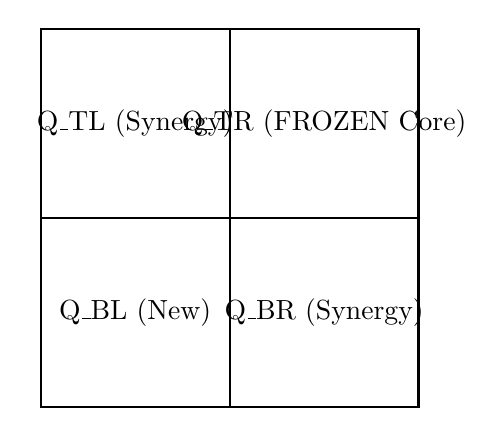
\begin{tikzpicture}[scale=0.8]
    \draw[thick] (0,0) rectangle (6,6);
    \draw[thick] (3,0) -- (3,6);
    \draw[thick] (0,3) -- (6,3);
    \node at (1.5,4.5) {Q\_TL (Synergy)};
    \node at (4.5,4.5) {Q\_TR (FROZEN Core)};
    \node at (1.5,1.5) {Q\_BL (New)};
    \node at (4.5,1.5) {Q\_BR (Synergy)};
\end{tikzpicture}
\caption{Quadrant topology of an expanded DGE weight matrix.}
\end{figure}

\section{RoPE-Invariant Head Expansion}

To preserve semantic integrity in Rotary Positional Embedding (RoPE) models, DGE expands width by adding \textbf{complete attention heads} ($d_{model} \leftarrow d_{model} + h \cdot d_{head}$) rather than individual dimensions. This preserves the frequency basis $\Theta$ for legacy heads.

\section{Experimental Results}

We evaluated DGE on a sequential skill acquisition task ("Count Up" then "Count Down") using shared token embeddings.

\subsection{Ablation Study}

To isolate the contribution of each component, we performed an extensive ablation study (V18-V26).

\begin{center}
\begin{tabular}{lccccc}
\toprule
\textbf{Configuration} & \textbf{Replay} & \textbf{Router} & \textbf{Init} & \textbf{Plasticity} & \textbf{Stability} \\
\midrule
Baseline (No DGE) & None & - & - & High (1.0) & Fail (16.0) \\
Strict Separation & None & MLP & Random & Fail (1.3) & Fail (16.4) \\
Hierarchical Gating & Yes & MLP Unigram & -4.0 & Low (50\%) & Low (50\%) \\
Soft Separation & Yes & MLP Unigram & 0.0 & Medium & Medium \\
\textbf{Directed Synergy} & \textbf{Asym.} & \textbf{Bigram} & \textbf{0.0} & \textbf{Success (1.0)} & \textbf{Success (1.98)} \\
\bottomrule
\end{tabular}
\end{center}

\subsection{Analysis}
\begin{itemize}
    \item \textbf{Strict Separation Failed (Leakage Creep):} Without Replay, microscopic leakage through the shared embedding space accumulated to destroy the old task.
    \item \textbf{Unigram Failed (Aliasing):} Hierarchical Gating with a Unigram router could not separate identical tokens used in different contexts.
    \item \textbf{Directed Synergy Succeeded:} The Bigram router resolved Aliasing, while Asymmetric Replay reinforced the separation boundary.
\end{itemize}

\section{Limitations}

While DGE solves the Plasticity-Stability Dilemma for our benchmarks, important limitations remain:

\begin{enumerate}
    \item \textbf{Contextual Overhead:} The Bigram Router requires $\mathbb{R}^{2d}$ input dimension, doubling the parameter count of the gating layer compared to a Unigram router.
    \item \textbf{Memory Footprint:} While computationally efficient, expanding the matrix physically consumes memory. Unlike LoRA, which adds small adapters, DGE adds full capacity.
    \item \textbf{Dependency on Replay:} Although reduced to 10\%, DGE still requires access to a replay buffer, which may raise privacy concerns in some applications.
\end{enumerate}

\section{Conclusion}

The Directed Synergy framework demonstrates that "Strict Separation" is insufficient for deep continual learning due to leakage and aliasing. By acknowledging these physical realities and employing \textbf{Contextual Gating} to resolve ambiguity and \textbf{Asymmetric Replay} to enforce boundaries, DGE offers a scientifically robust solution for extending Large Language Models.

\bibliographystyle{plain}
\begin{thebibliography}{9}
\bibitem{gge} Jansen, S. (2024). Gated Ghost Expansion: A Unified Theory for Lossless Dimension Extension in RoPE-based LLMs.
\bibitem{rope} Su, J., et al. (2021). RoFormer: Enhanced Transformer with Rotary Position Embedding.
\bibitem{ewc} Kirkpatrick, J., et al. (2017). Overcoming catastrophic forgetting in neural networks.
\end{thebibliography}

\end{document}
